\documentclass[letterpaper, 12pt, titlepage]{article}
%=======Unpackage Things===============
\usepackage{array}
\usepackage{color}
\usepackage{colortbl}
\usepackage{algorithm}
\usepackage[noend]{algpseudocode}
\usepackage{graphicx}
\usepackage{amsmath}
\usepackage{amsthm}
\usepackage{listings}
%\usepackage{fullpage}
\usepackage{epsfig}
\usepackage{amsmath}
\usepackage{latexsym}
\usepackage{amssymb}
\usepackage{ulem}
\usepackage{amstext}
\usepackage{float}
\usepackage{mathrsfs}
\usepackage{mathtools}
\usepackage{geometry}
\usepackage{setspace}
\usepackage{enumerate}
\DeclarePairedDelimiter\ceil{\lceil}{\rceil}
\newcommand{\PreserveBackslash}[1]{\let\temp=\\#1\let\\=\temp}
\newcolumntype{C}[1]{>{\PreserveBackslash\centering}p{#1}}
\newcolumntype{R}[1]{>{\PreserveBackslash\raggedleft}p{#1}}
\newcolumntype{L}[1]{>{\PreserveBackslash\raggedright}p{#1}}

\begin{document}
%==title==
\title{COMP6521}
\setcounter{tocdepth}{2}
\newpage
\begin{center}
    {\bf\large COMP6321 Project Proposal}

    $\mathcal{C}$orrespondence $\mathcal{F}$inding in 3D $\mathcal{R}$econstruction

     \vspace{1cm}
\uuline{
    Student: Qing Gu  \hspace{5cm}
    Student ID: 6935451}
    \vspace{0.1cm}
\end{center}

3D reconstruction with stereo requires finding correspondence in 3D scene, which is usually one of the most challenging problem. This project is looking for a machine learning algorithm to find correspondence in two pictures taken by left and right lens of stereo camera.
\begin{figure}[H]
\centering
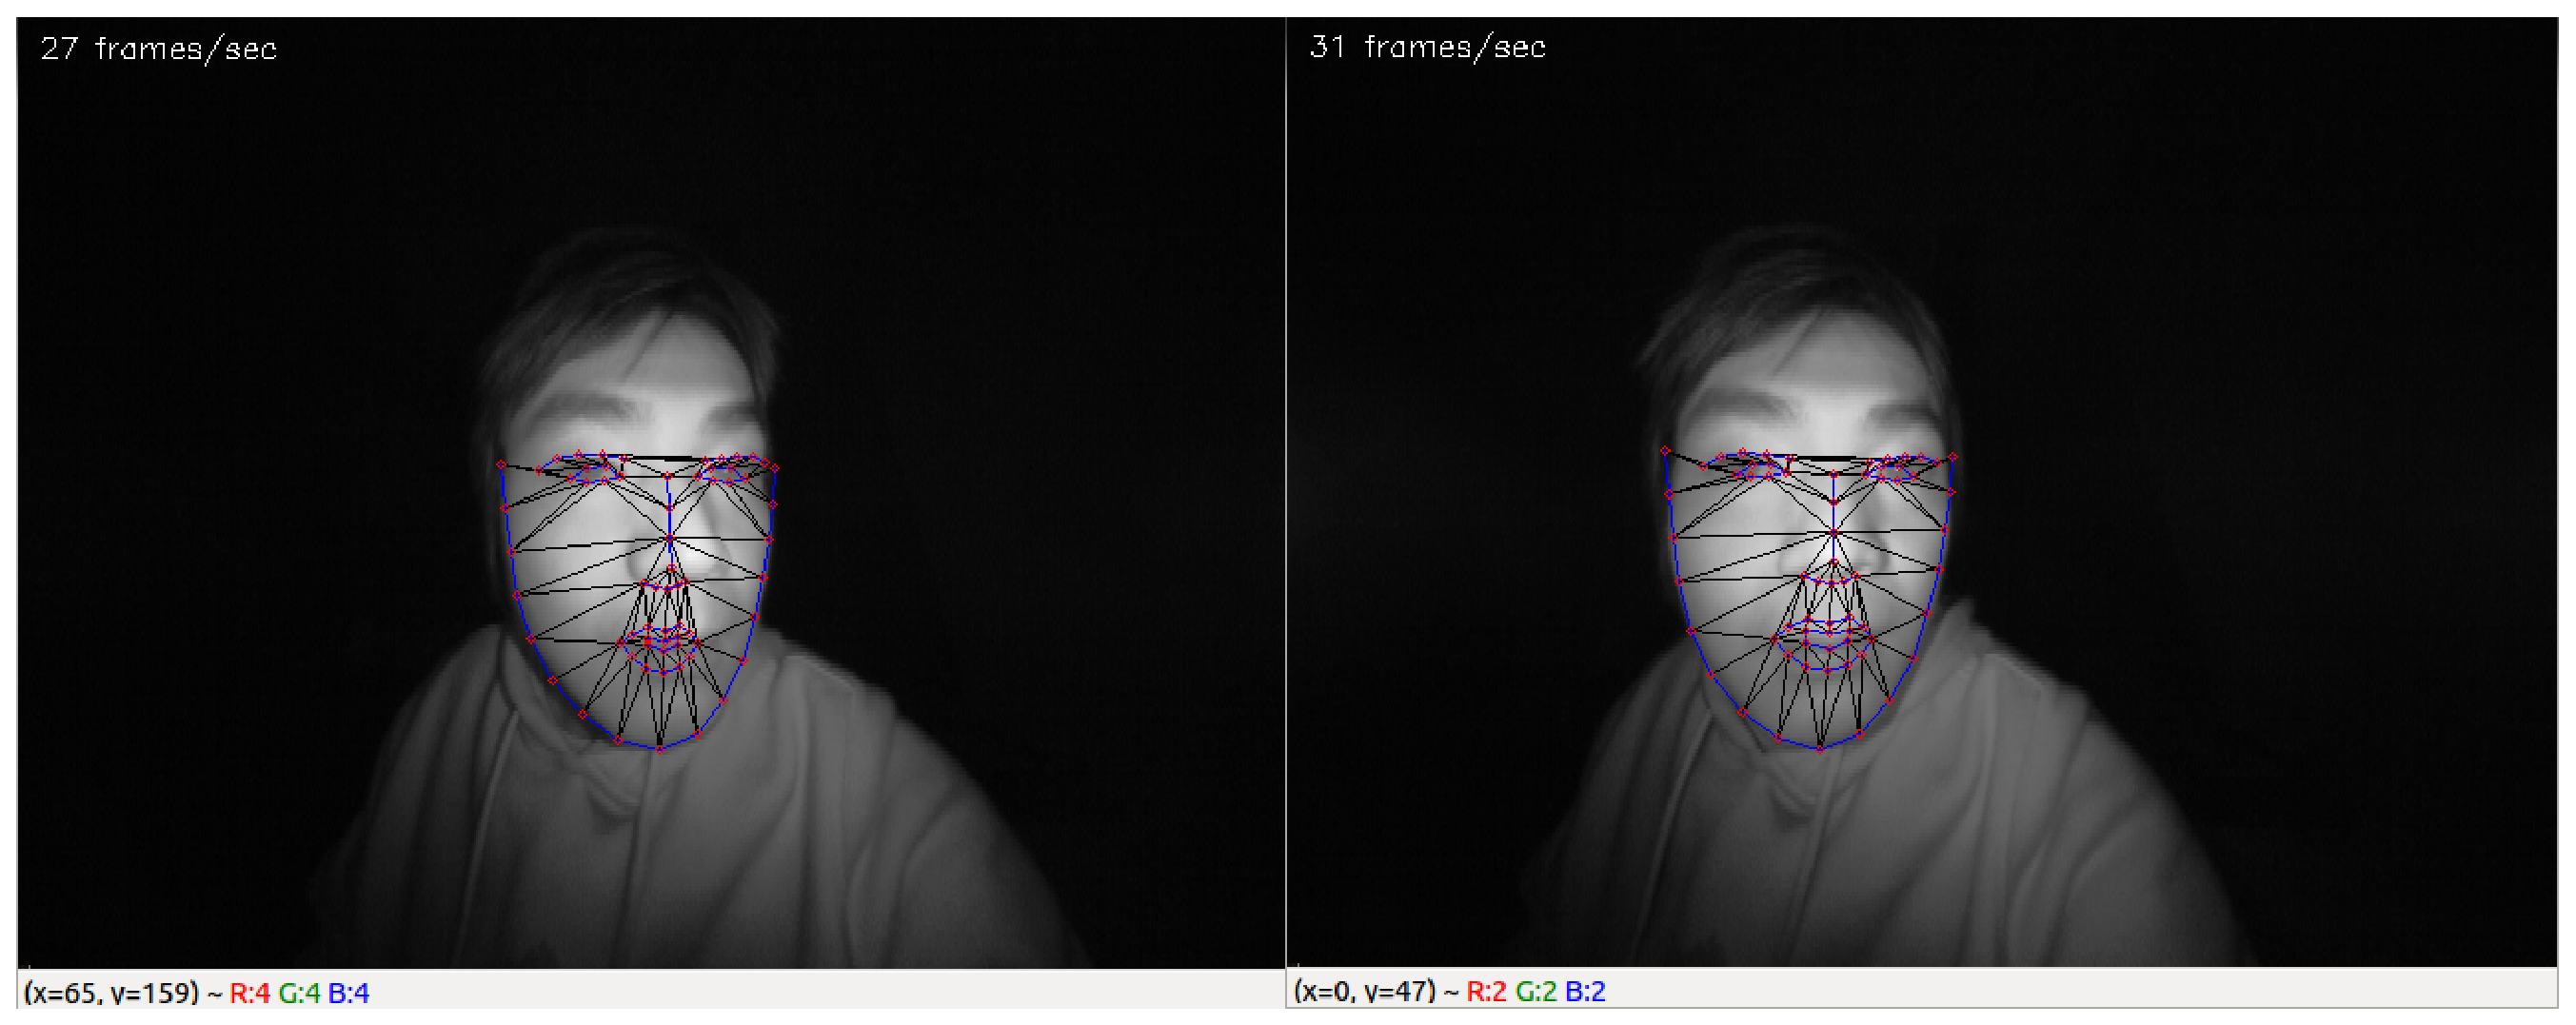
\includegraphics[width=12cm]{stereoImage.eps}
\caption{Stereo Image with Face Recoginition}
\label{Q1}
\end{figure}

The goal of the project is to reconstruct face anchor point in 3D space using stereo camera provided by Leap Motion. In order to find correspondent points in two images, a face recognition algorithm is used. The technique is mentioned in the following paper. 

http://ci2cv.net/static/papers/2013\_AFGR\_Cheng.pdf








%\begin{spacing}{0.1}
%\noindent\hfil\rule{0.8\textwidth}{.1pt}\hfil

%\noindent\hfil\rule{0.8\textwidth}{.1pt}\hfil
%\end{spacing}


  

        




\end{document}
